\section{Open loop analysis}

\subsection{}
The definition of crab angle from REF:BEARD is
\begin{equation}\begin{aligned}
\chi_c \triangleq \chi - \psi
\end{aligned}\end{equation}
where $\chi$ is the course and $\psi$ is the heading. Since the wind speed is assumed zero, the sideslip $\beta = \chi_c$ and so
\begin{equation}\begin{aligned}
\beta = \chi - \psi.
\end{aligned}\end{equation}

\subsection{}
\begin{figure}[ht]
	\centering
	\begin{subfigure}[b]{0.45\textwidth}
		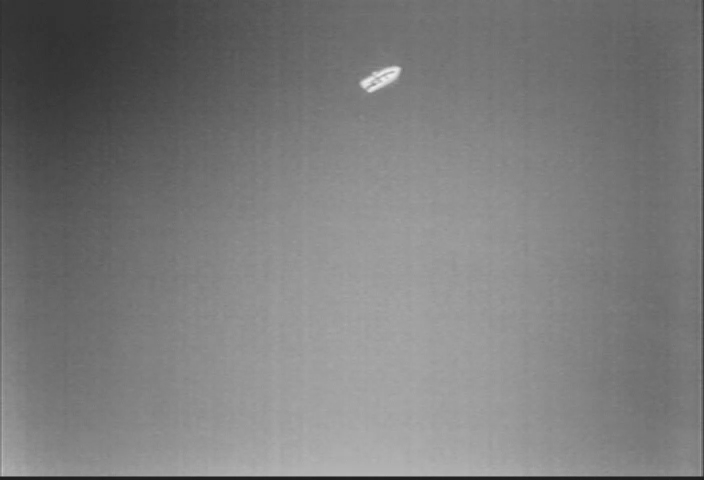
\includegraphics[width=\textwidth]{fig1}
		\caption{caption..}
		\label{fig:2a}
	\end{subfigure}
	~ %add desired spacing between images, e. g. ~, \quad, \qquad, \hfill etc.
	%(or a blank line to force the subfigure onto a new line)
	\begin{subfigure}[b]{0.45\textwidth}
		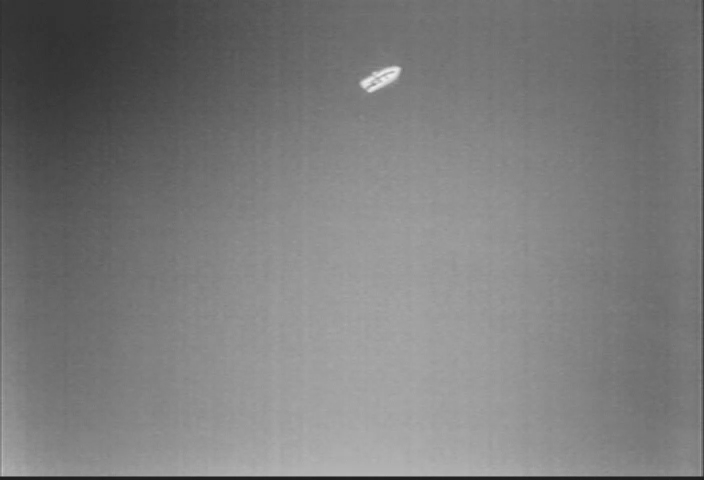
\includegraphics[width=\textwidth]{fig1}
		\caption{caption..}
		\label{fig:2b}
	\end{subfigure}
	\begin{subfigure}[b]{0.45\textwidth}
		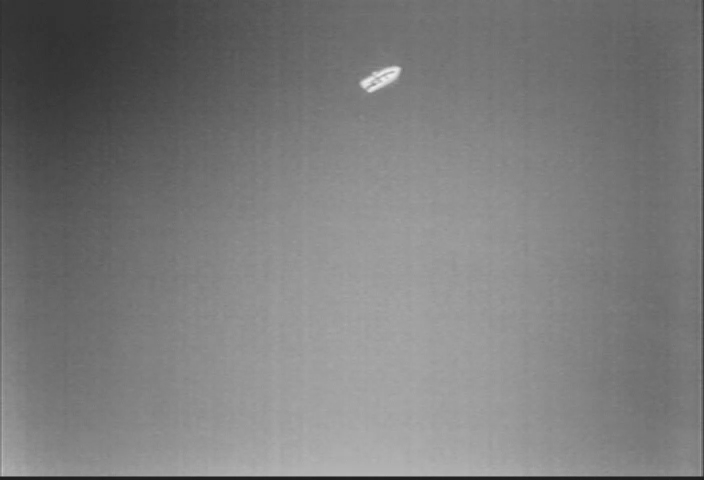
\includegraphics[width=\textwidth]{fig1}
		\caption{caption..}
		\label{fig:2c}
	\end{subfigure}
	\begin{subfigure}[b]{0.45\textwidth}
		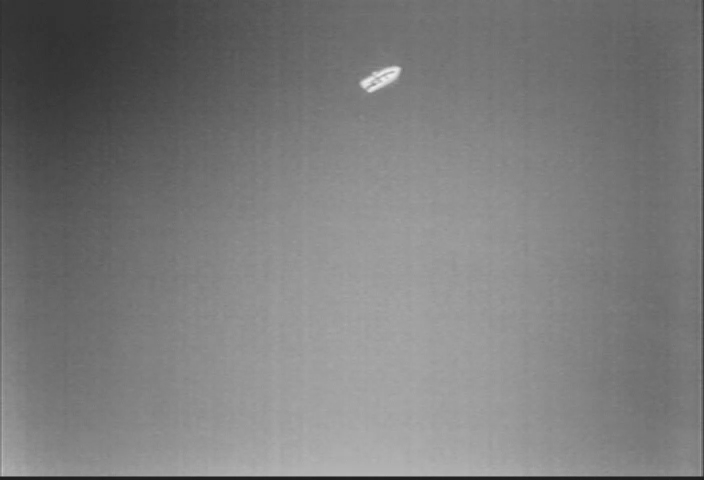
\includegraphics[width=\textwidth]{fig1}
		\caption{caption..}
		\label{fig:2d}
	\end{subfigure}
	\caption{Caption for all figures}\label{fig:2}
\end{figure}
